A primeira simulação feita foi simplesmente executar a dinâmica do por um 
determinado número de iterações. Iniciamos posicionando as moléculas no espaço 
2D nos centros de malha regular com espaçamentos de $L/\sqrt{N}$ onde $L$ é o tamanho da 
caixa e $N$ o número de partículas e então adicionando um pequeno deslocamento aleatório
em cada uma delas. 

A figura(\ref{fig:posicoes-iniciais-a}) abaixo mostra esse posicionamento inicial definido para os corpos.

\begin{figure}[h!]
    \centering
    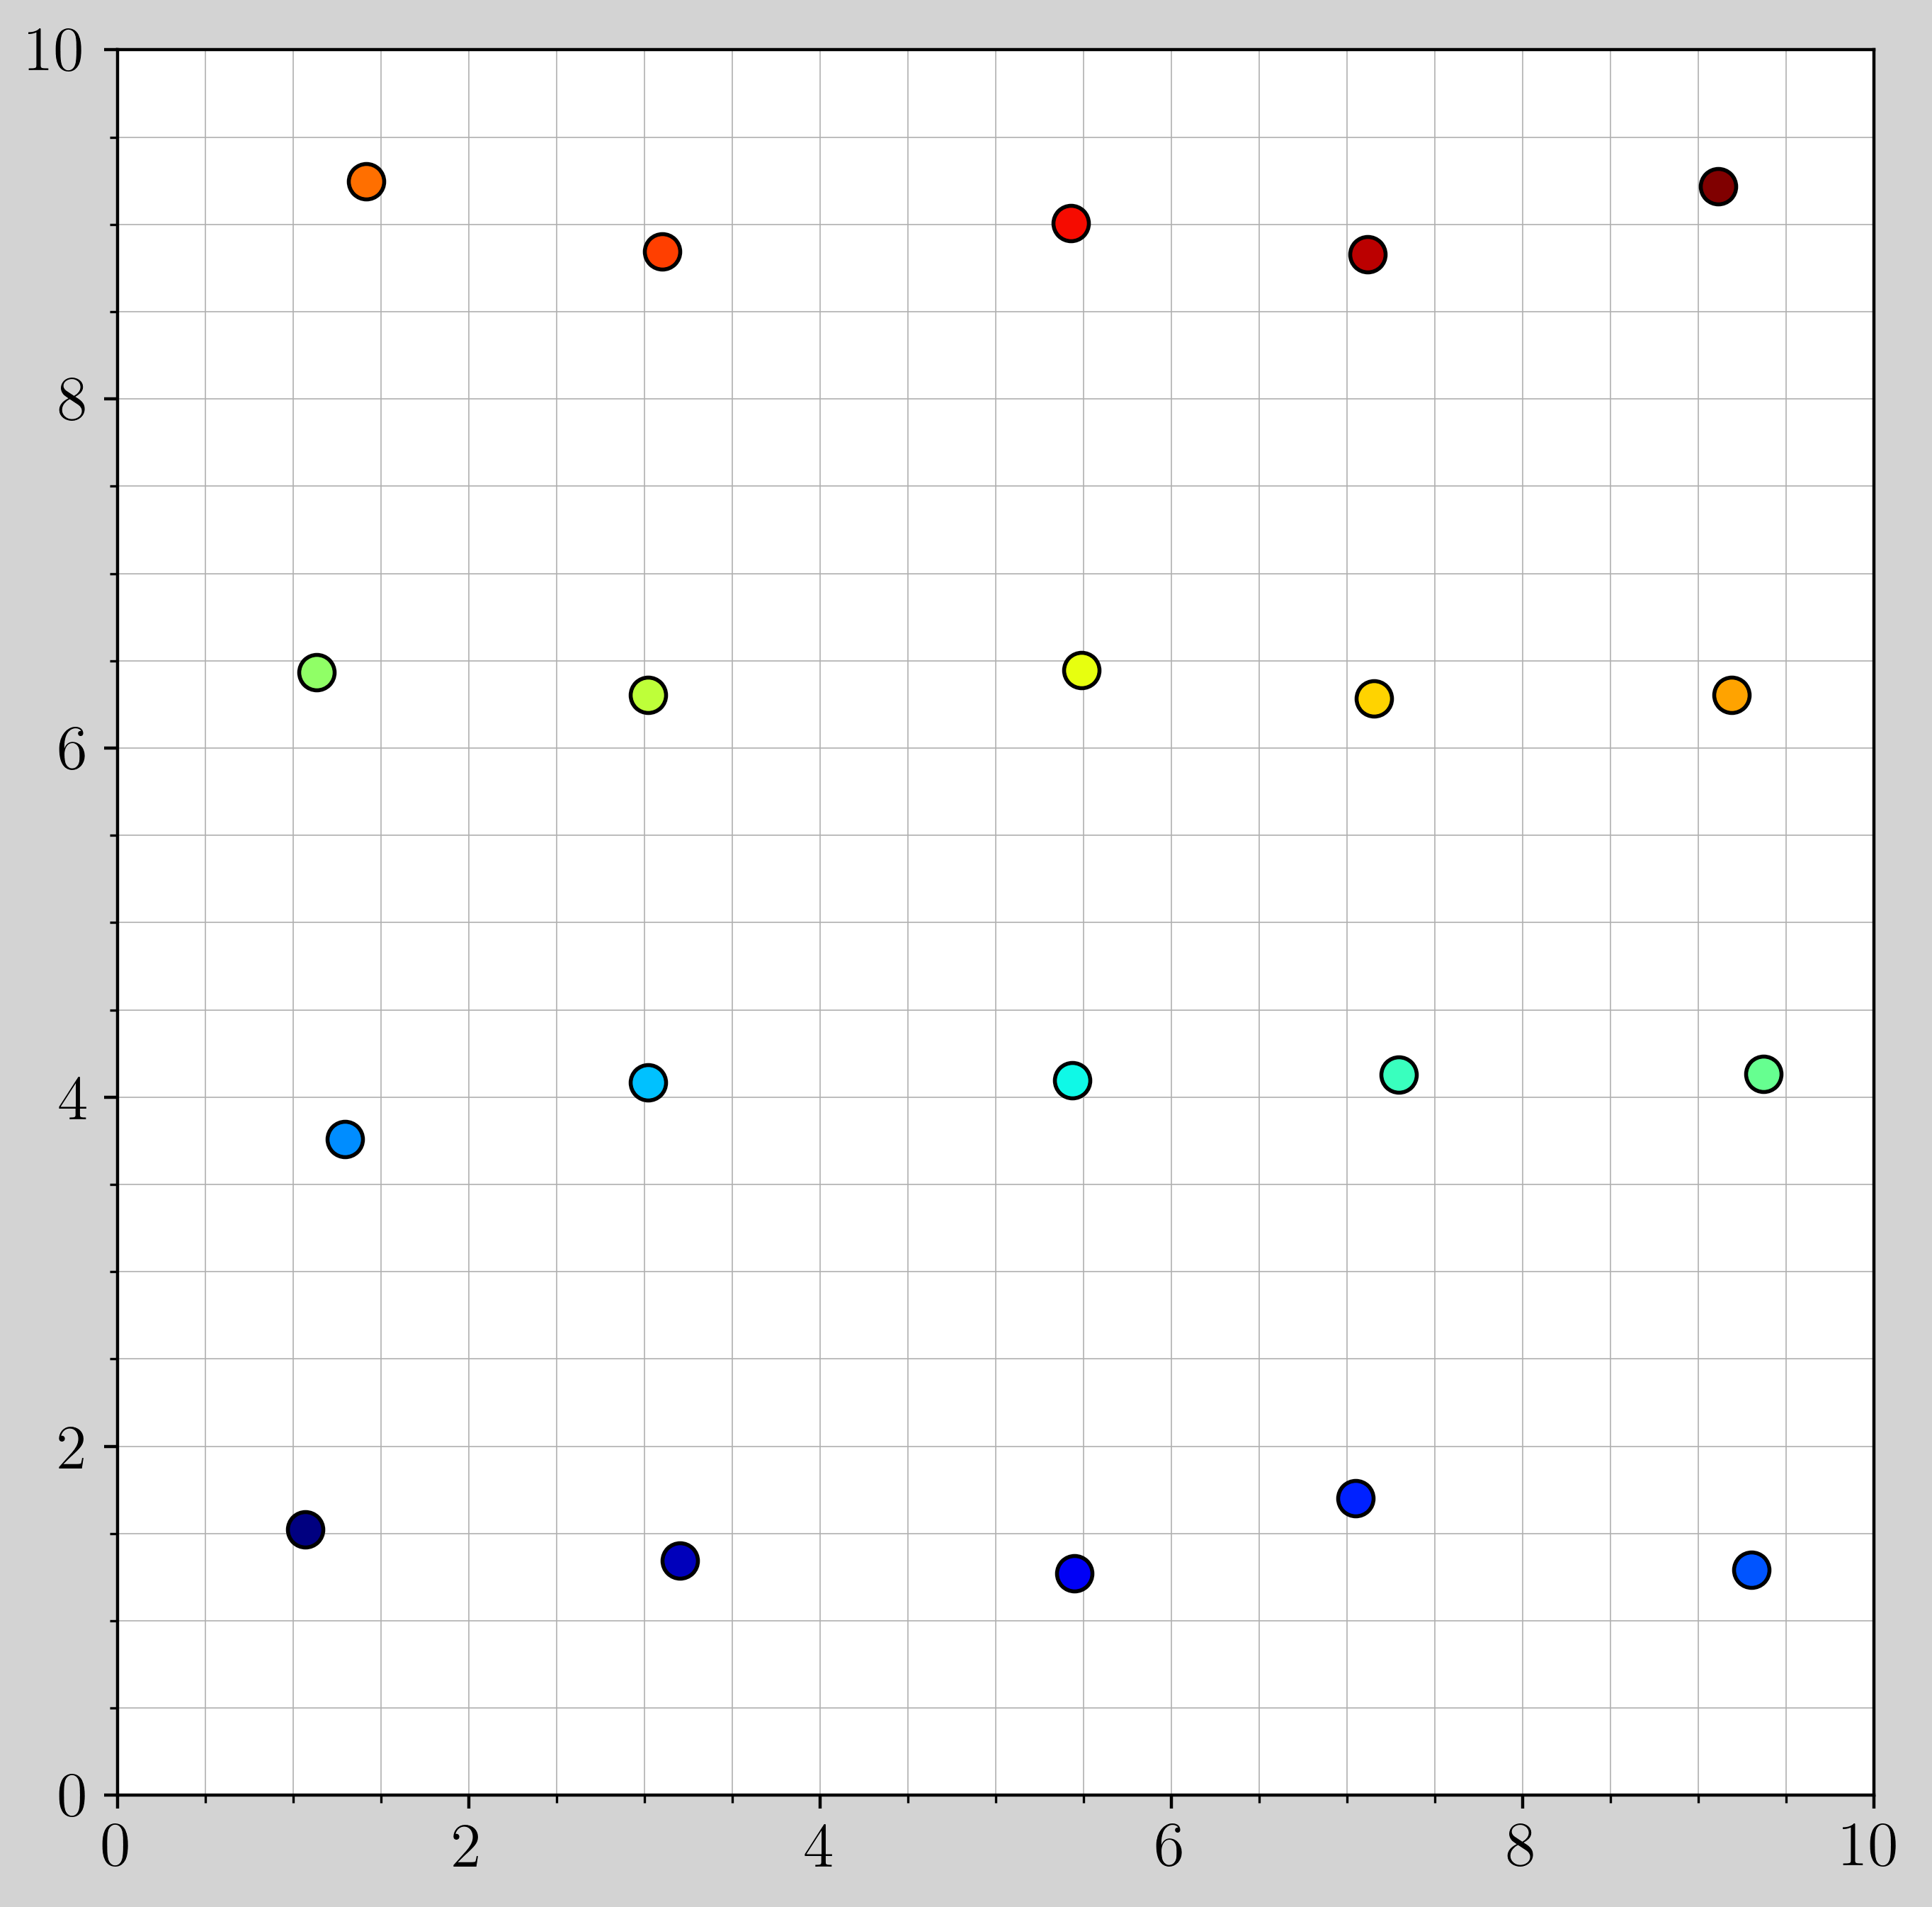
\includegraphics[width=0.3\linewidth]{tarefa-A/posicoes-iniciais.png}
    \caption{Posições iniciais das partículas.}
    \label{fig:posicoes-iniciais-a}
\end{figure}

a figura abaixo mostra o  ``rastro'' que as partículas fazem para uma simulação de $500$ iterações. 
Os dados considerados são somentes os iterações multiplas de $3 \Delta t$. Além dessa figura 
também foi gerado uma animação em \verb|gif| da dinâmica molecular, é o arquivo 
localizado na pasta \verb|gráficos/tarefa-A/| entitulado \verb|evolucao.gif|.  

\begin{figure}[h!]
    \centering 
    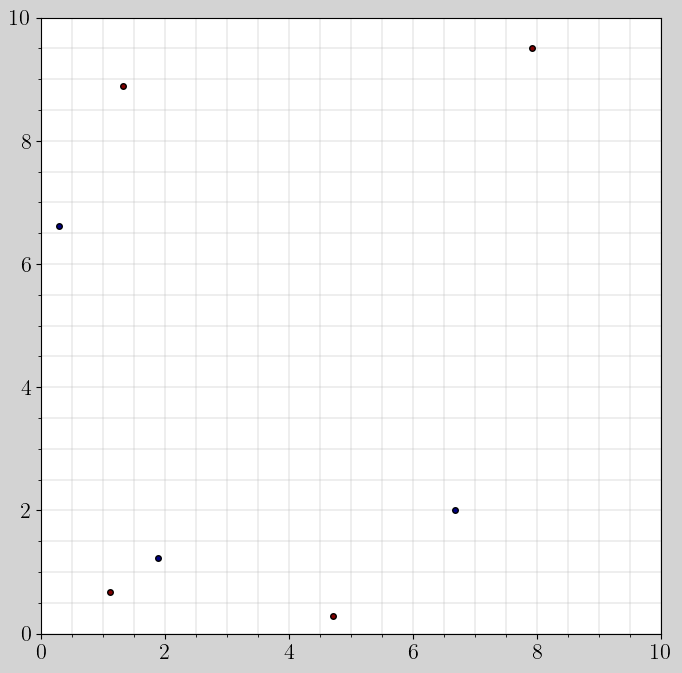
\includegraphics[width=0.3\linewidth]{tarefa-A/posicoes-finais.png}
    \label{fig:posicoes-finais-a}
    \caption{Coordenadas das partículas projetadas à cada $3 \Delta t$.}
\end{figure}


Também foi construido também um gráfico da energia(\ref{fig:energia-a}) total do sistema para essa simulação.
podemos notar que há variações grandes na energia, mas ela ainda se mantem oscilando em torno de um valor, isso era o esperado. 
Essa variação pode ser devido ao uso de condições periodicas de contorno utilizadas, já que o numéro de partículas e densidade de partículas 
é relativamente pequeno.

\begin{figure}[h!]
    \centering 
    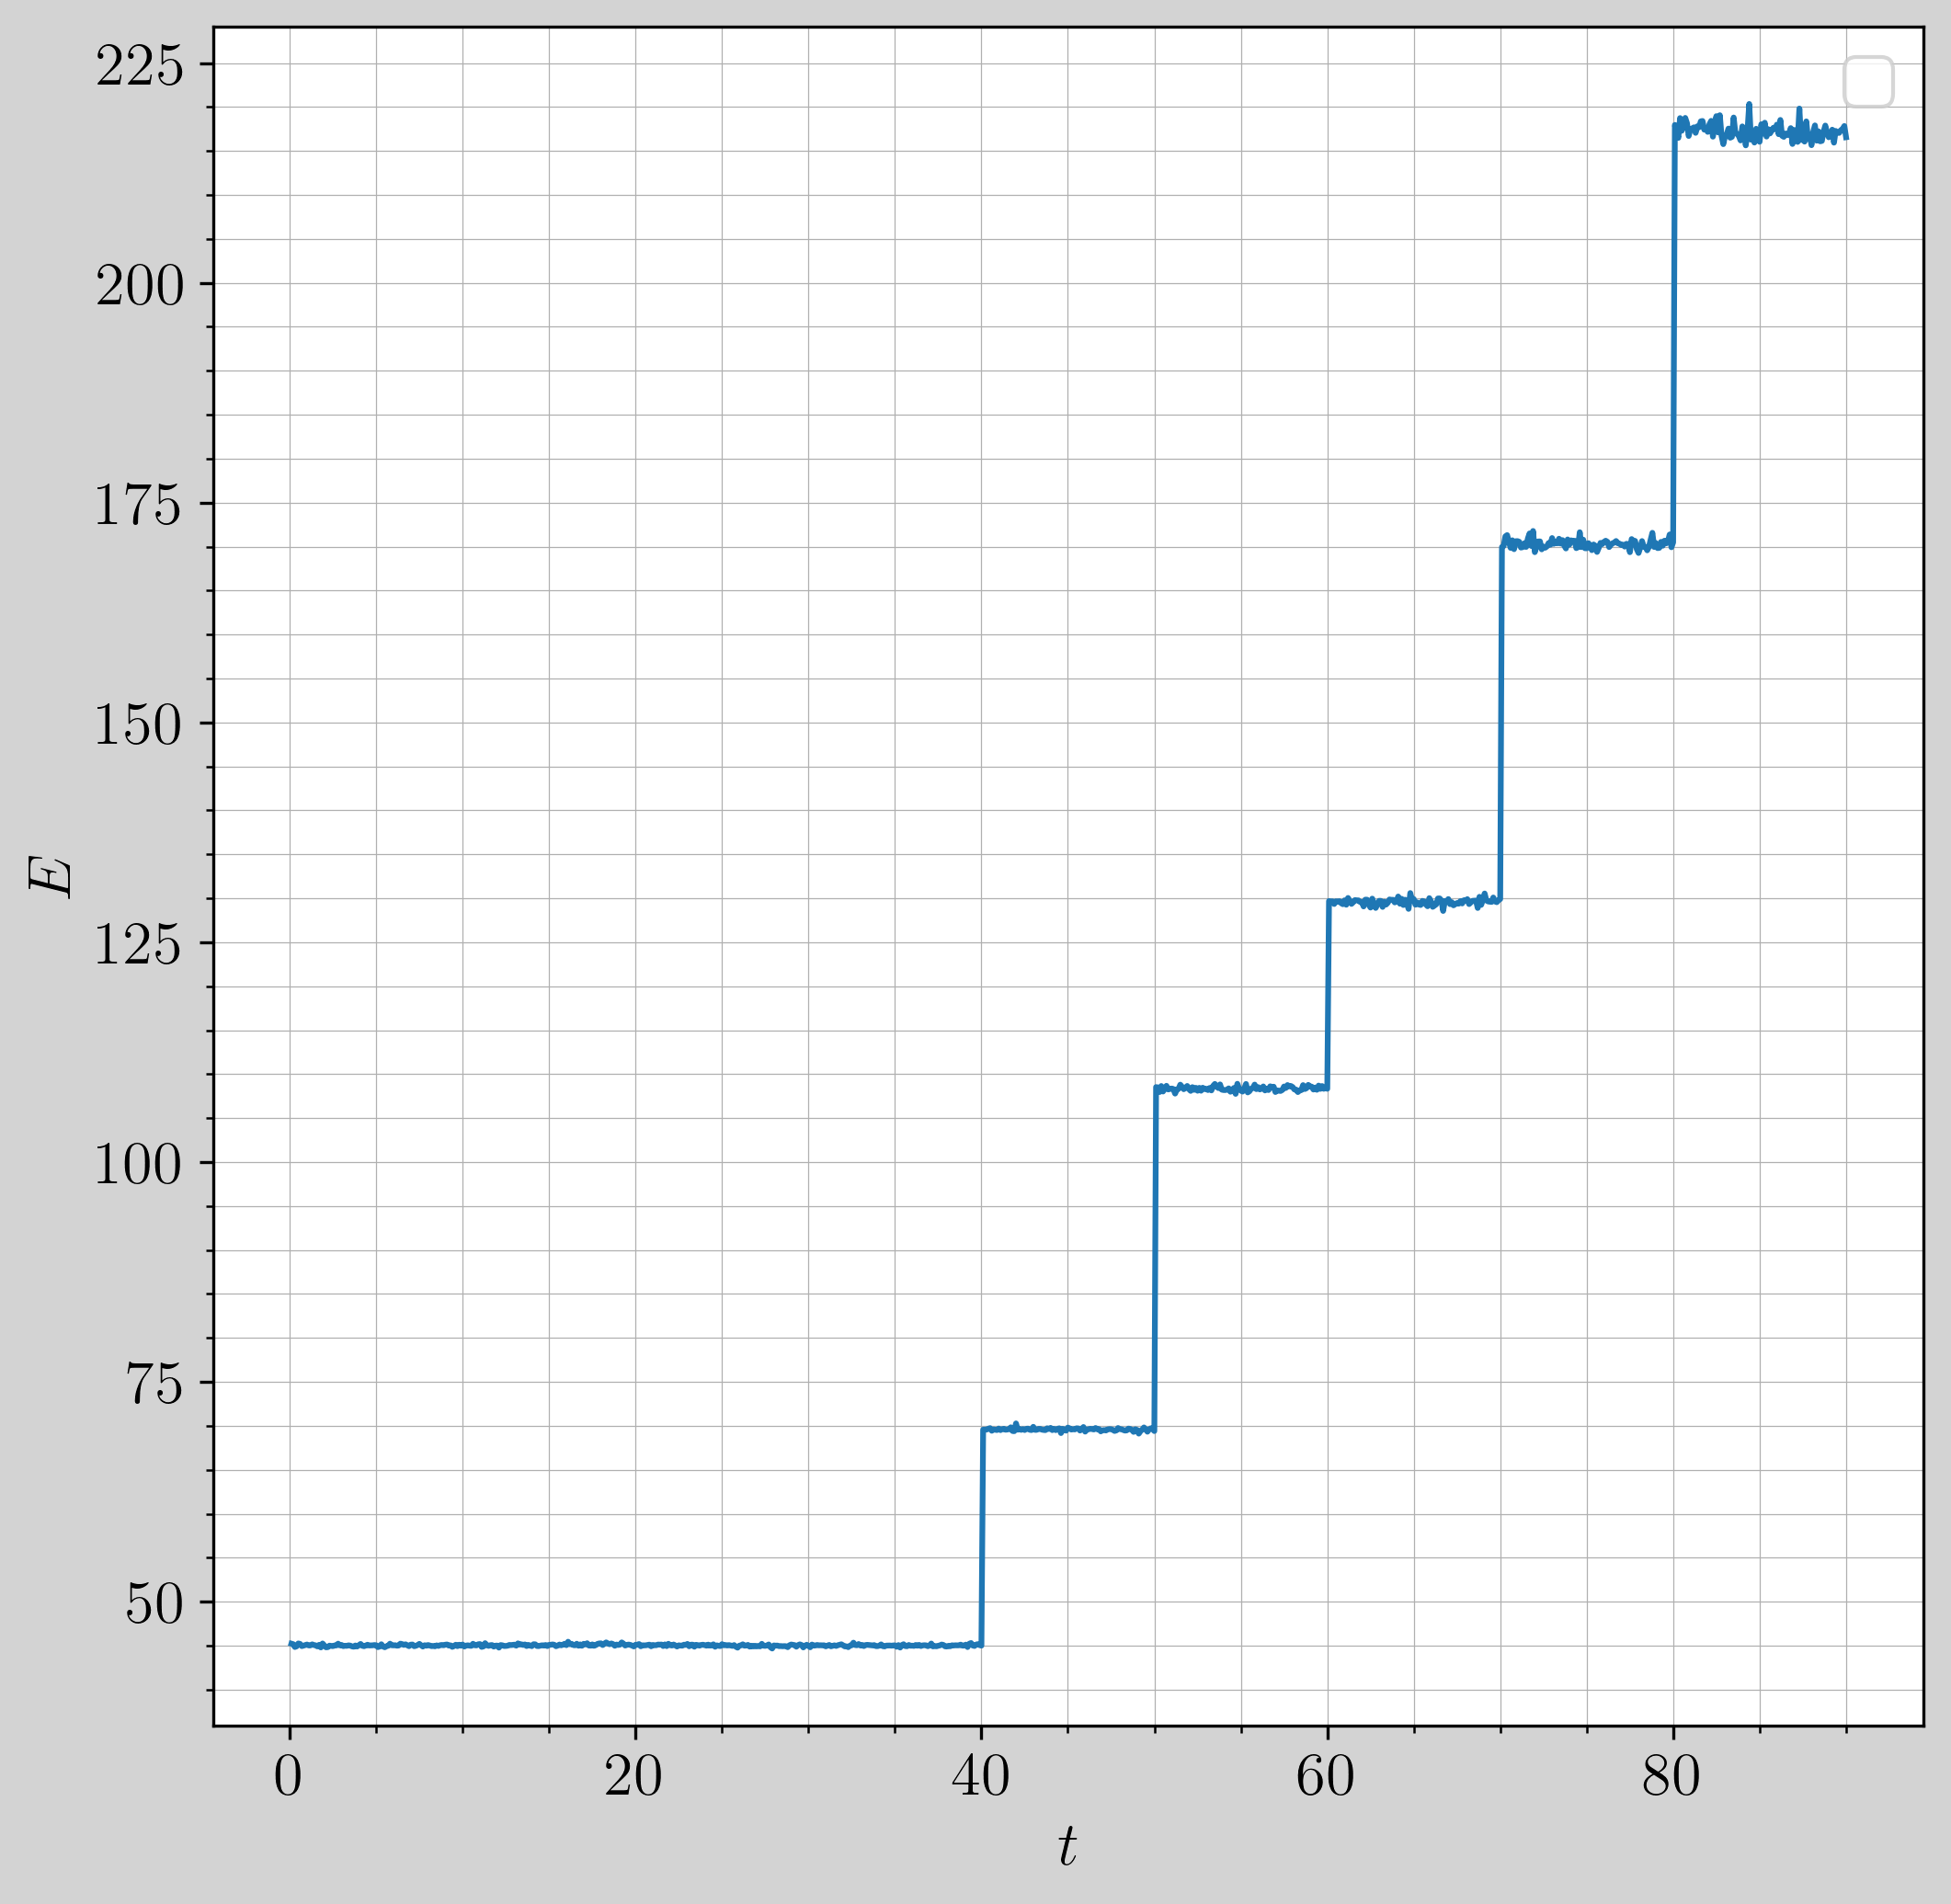
\includegraphics[width=0.3\linewidth]{tarefa-A/energia.png}
    \caption{Energia do sistema à cada $3 \Delta t$.}
    \label{fig:energia_a}
\end{figure}

\clearpage
\subsection{Implementação - Simulação A}
\label{ssec:codigoA}
O código abaixo está no diretório \verb|tarefa-a/| e contém 
as simulações referentes às tarefas A, B e parte da D.
\begin{minted}{fortran}
    ! Tarefas A, B e parte da D
    implicit real*8(a-h, o-y)
    parameter (pi = acos(-1.e0))
    dimension r_prev(20, 2)
    dimension r_curr(20, 2)
    dimension r_next(20, 2)
    dimension v(20, 2)
    dimension r(20, 20)
    dimension acc(2)
    L = 10
    rL = 10d0
    N = 20

    ! Tarefa A 
    open(unit = 99, file="saidas/tarefa-A/parametros.dat")
    open(unit = 1,  file="saidas/tarefa-A/posicoes-iniciais.dat")
    open(unit = 3,  file="saidas/tarefa-A/evolucao-posicoes.dat")
    ! Tarefa B 
    open(unit = 5,  file="saidas/tarefa-B/velocidades.dat")
    open(unit = 6,  file="saidas/tarefa-B/evolucao-posicoes.dat")
    ! Tarefa D
    open(unit = 9,  file="saidas/tarefa-D/temperatura-b.dat")
    
    dt = 0.02
    v0 = 1.0
    write(99, *) N, L, v0, dt
    close(99)
    ! Defining # rows/columns 
    n_cols = ceiling(sqrt(N*1d0))
    n_rows = ceiling((N*1d0)/(n_cols*1d0)) 
    
    ! Spacing 1/4 
    x_spacing = L/(1d0*n_cols)
    y_spacing = L/(1d0*n_rows)
    spacing = min(x_spacing, y_spacing)/4.0 
    
    ! Centering in the grid
    x_offset = x_spacing / 2.0 
    y_offset = y_spacing / 2.0
    call srand(562369)
    
    k = 1 
    do j = 1, n_rows 
          do i = 1, n_cols 
                r_curr(k, 1) = (i-1)*x_spacing+x_offset
                r_curr(k, 2) = (j-1)*y_spacing+y_offset
                
                r_curr(k, 1) = r_curr(k,1)+(rand())*spacing
                r_curr(k, 2) = r_curr(k,2)+(rand())*spacing
                theta = 2*pi*rand()
                v(k, 1) = v0*cos(theta)
                v(k, 2) = v0*sin(theta)
                
                r_prev(k, 1) = r_curr(k, 1) - v(k, 1) * dt 
                r_prev(k, 2) = r_curr(k, 2) - v(k, 2) * dt 
                k=k+1
          end do 
    end do

    do i = 1, N
          write(1, *) r_curr(i, 1), r_curr(i, 2) 
          write(3, *) 0d0, r_curr(i,1), r_curr(i, 2)
    end do
    close(1)

    DB = 1.0
    ! Dynamics 
    do k = 1, 5000

          t = k * dt 

          acc(1) = 0d0 
          acc(2) = 0d0

          do i = 1, N 
                acc(1) = 0d0 
                acc(2) = 0d0
                do j = 1, N 
                      if(i /= j) then
                           call compute_acc(N,i,j,L,r_curr,acc,r)
                      end if
                end do 
                ! UPDATE POSITIONS
                r_next(i,1) = 2*r_curr(i,1)-r_prev(i,1)+acc(1)*(dt**2)
                r_next(i,2) = 2*r_curr(i,2)-r_prev(i,2)+acc(2)*(dt**2) 

                ! APPLY PBC
                r_next(i,1) = mod(r_next(i,1)+rL, rL)
                r_next(i,2) = mod(r_next(i,2)+rL, rL)

                delta_r_x = delta_pbc(r_next(i,1),r_prev(i,1),L)
                delta_r_y = delta_pbc(r_next(i,2),r_prev(i,2),L)

                ! UPDATE VELOCITIES using adjusted displacements
                v(i, 1) = delta_r_x / (2 * dt)
                v(i, 2) = delta_r_y / (2 * dt)
          end do

          r_prev(:, 1) = r_curr(:, 1)
          r_prev(:, 2) = r_curr(:, 2)
          
          r_curr(:, 1) = r_next(:, 1)
          r_curr(:, 2) = r_next(:, 2)
          
          if(k < 200) then 
                E = 0d0
                call compute_energy(N, L, v, r_curr, E, r)
                write(19,*) k, E
          end if

          ! TAREFA A 
          if(mod(k, 3) == 0 .and. k < 400) then
                do i = 1, N 
                      write(3,*) k, r_curr(i,1),r_curr(i, 2)
                end do
          end if

          ! Tarefa B & D 
          if(mod(k, 20) == 0) then
                do i = 1, N
                      v_mag = sqrt(v(i,1)**2+v(i,2)**2)
                      write(5,*) k, v_mag, v(i,1), v(i,2)
                      write(9,*) .5d0 * v_mag**2
                      write(6,*) k, r_curr(i,1),r_curr(i, 2)
                end do
          end if
    end do
    close(3)
    close(5)
    close(6)
    close(9)
    close(15) 

    end
    ! Submodules for molecular dynamic simulations
    ! Velocity delta 
    function delta_pbc(r_next, r_prev,L)
          implicit real*8(a-h, o-y)
          delta_pbc = r_next - r_prev
          delta_pbc = delta_pbc - L * nint(delta_pbc / L)
    end function delta_pbc

    subroutine initialize_particles(N, L, r_curr,r_prev, v, v0)
          implicit real*8(a-h, o-y)
          dimension r_prev(20, 2)
          dimension r_curr(20, 2)
          dimension v(20, 2)
         
          ! Defining # rows/columns 
          n_cols = ceiling(sqrt(N*1d0))
          n_rows = ceiling((N*1d0)/(n_cols*1d0)) 
          
          ! Spacing 1/4 
          x_spacing = L/(1d0*n_cols)
          y_spacing = L/(1d0*n_rows)
          spacing = min(x_spacing, y_spacing)/4.0 
          
          ! Centering in the grid
          x_offset = x_spacing / 2.0 
          y_offset = y_spacing / 2.0
          call srand(562369)

          k = 1 
          do j = 1, n_rows 
                do i = 1, n_cols 
                      r_curr(k, 1) = (i-1)*x_spacing+x_offset
                      r_curr(k, 2) = (j-1)*y_spacing+y_offset
                      
                      r_curr(k, 1) = r_curr(k,1)+(rand())*spacing
                      r_curr(k, 2) = r_curr(k,2)+(rand())*spacing

                      theta = 2*pi*rand()
                      v(k, 1) = v0*cos(theta)
                      v(k, 2) = v0*sin(theta)
                      
                      r_prev(k, 1) = r_curr(k, 1) - v(k, 1) * dt 
                      r_prev(k, 2) = r_curr(k, 2) - v(k, 2) * dt 
                      k=k+1
                end do 
          end do
    end subroutine initialize_particles

    ! Updates acceleration a = ax, ay 
    ! between particle i and all others
    subroutine compute_acc(N,i,j,L,r_curr,acc, r)
          implicit real*8(a-h, o-y)
          dimension r_curr(20, 2)
          dimension acc(2)
          dimension r(20, 20)
          epsilon = 1e-3

          dx = r_curr(i, 1) - r_curr(j, 1)
          dy = r_curr(i, 2) - r_curr(j, 2)

          dx = dx - L * nint(dx / L)
          dy = dy - L * nint(dy / L)

          r_ij = sqrt(dx**2 + dy**2)
          
          r(i, j) = r_ij 
          r(j, i) = r_ij

          if(r_ij > epsilon .and. r_ij <= 3d0) then 
                F = 24.0 * (2d0/r_ij**13 - 1d0/r_ij**7)
                acc(1) = acc(1) + F * dx / r_ij 
                acc(2) = acc(2) + F * dy / r_ij
          end if 
    end subroutine compute_acc

    subroutine compute_energy(N, L, v, r_curr, E, r)
          implicit real*8(a-h, o-y)
          dimension v(20, 2)
          dimension r_curr(20, 2)
          dimension r(20, 20)
          
          epsilon = 1e-3
          Tk = 0d0
          do i = 1, N
              Tk = Tk + 0.5 * (v(i, 1)**2 + v(i, 2)**2)
          end do
          U = 0d0
          do i = 1, N
            do j = i + 1, N
                r_ij = r(i, j)

                if (r_ij > epsilon .and. r_ij <= 3d0) then
                    U = U + 4 * (r_ij**(-12) - r_ij**(-6))
                end if
            end do
          end do
          E = Tk + U
    end subroutine
\end{minted}
\clearpage